\chapter{Design and Implementation}

\section{Development Methodology}
Software development methodologies break the development of a piece of software down into a number of phases with the aim of improving design and code quality as well as aiding in project management. There are a large number of different development methodologies, although they can typically be classified as either sequential, also called waterfall, or cyclical, also called spiral. The choice of which method to use will depend on the specifics of the software project as well as developer preference and team size.

\subsection{Sequential}
The sequential, or waterfall, approach uses a number of strict, sequential phases for developing software; each phase must be completed before the next phase can begin. Fig. \ref{fig:waterfall} shows the typical structure of this methodology.
\begin{figure}[tp]
   \begin{center}
     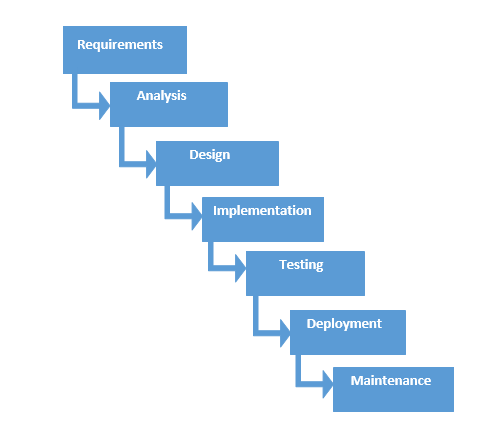
\includegraphics{Figures/waterfall.png}
   \end{center}
   \caption[Waterfall development methodology]{Waterfall development methodology \parencite{Naveen}}
   \label{fig:waterfall}
\end{figure}
\\This approach works well for projects were the requirements are strictly defined, the project's subject area well known and the technologies involved well understood by the developers. In this case, the software can be designed well from the start, so there is little need for iterative development. If the project's requirements are likely to change, or the subject area and technologies are ill-understood or new then a waterfall approach is inappropriate. The rigid structure of the waterfall method does not allow requirements to be easily changed, or poor design choices corrected; in order to change requirements or correct poor design the whole development process must be started again, as there is no method of feedback between development phases.

\subsection{Cyclical}
Cyclical approaches, as the name suggests, develop software using iterative cycles. At the start of each cycle requirements and design are set and at the end, a working software prototype is produced. This prototype is used as feedback for the next cycle, adjusting the requirements and correcting design mistakes and issues as necessary. These methods counteract the disadvantages of the waterfall approach; by using an iterative approach it is easy to add or change requirements or redesign areas of the project.
\\There are many development methods which are derived from a cyclic approach, including Rapid Application Development (RAD) and Scrum.
\\RAD is a development method which favours rapid prototyping with minimal planning. Since there is less focus on planning at each iteration it is extremely easy to incorporate design and requirement changes. Prototype development will start earlier than other methods and this enables issues to be caught early, and the design to be altered appropriately. There is a requirement when using RAD of skilled and experience developers and designers, as the prototypes  developed must be reusable so as to avoid wasting time.
\\Using Scrum, a project is broken down into sprints and each sprint is timeboxed with a duration, i.e. 24 hours, 4 weeks. At the end of each sprint a working prototype is produced and as the sprints are completed the project is designed and developed over time.

\subsection{Chosen Methodology}
For this project, cyclical methods were preferred over waterfall. This was partly due to the author's preference for cyclical methods and partly because there were some unknowns, particularly related to rendering, that made rigidly designing the system difficult. Using the more agile cyclical methods allowed for some investigative work before finalising the system design.
\\In particular, RAD was chosen as the development methodology.

\section{Development}
Since RAD was the chosen development methodology, the artefact was developed over several cycles.

\subsection{First Cycle}
In the first cycle the Mass-Spring model was implemented. Springs were implemented using the Hooke equation (Equation \ref{eq:hooke equation}) to calculate the internal spring force with linear damping as an additional internal force using Equation \ref{eq:spring damping}. Gravity, implemented as Equation \ref{eq:gravity}, was the only external force. Rendering of the cloth was also implemented.
\\Table \ref{tab:cycle 1 require} shows the initial requirements of the first development cycle.
\begin{table}[tp]
   \begin{minipage}{\textwidth}
      \begin{center}
         \begin{tabular}{c|c}
           Requirement & Type\\
           \hline
           Must model cloth using the Provot Mass-Spring model & Functional\\
           Must be able to render cloth to the screen & Functional\\
           Must be able to pin particles so they are unaffected by forces & Functional\\
           Must perform in real time& Non-functional\\
         \end{tabular}
      \end{center}
   \end{minipage}
   \caption{First cycle requirements}
   \label{tab:cycle 1 require}
\end{table}
\\\\Before designing this cycle, an initial investigation into the rendering component was carried out, as the choice between DirectX11 or OpenGL would affect the design of the system.
\\As this project is not concerned with rendering cloth, but simulating it, it was decided that the cloth would be rendered as a mesh of lines, representing the structural and shear springs (as in Figs \ref{fig:structural and shear} and \ref{fig:super-elasticity}). Since the positions of the particles, and therefore vertices, will change over time, a DirectX11 implementation would have to use a dynamic vertex buffer and remap the vertex data every frame. This is not an issue in OpenGL, since it is possible to draw vertices directly with the glVertex3f function. It was unknown by the author what the cost of this remapping would be so simple OpenGL and DirectX11 implementations were created and their performance compared. For a 500 by 500 mesh, with a debug build, the OpenGL implementation rendered the structural and shear springs at 80FPS and the DirectX11 version at 450FPS. Hence, DirectX11 was chosen as the rendering language. It should be noted that the OpenGL implementation was very naive, due to the author's inexperience, and this is most likely the reason for the poor performance. It is probable that a more robust implementation, using more advanced features, would perform much more closely to the DirectX11 implementation.
\\\\The initial design can be seen in Fig \ref{fig:phase1 initial}; the rendering component, constructors, accessors and mutators have been excluded for brevity. 
\\Since DirectX11 was the rendering language, DirectXMath types were used for the key variables in the Particle class. This gives performance gains over manually implementing a 3-dimensional vector and functions, as the functions that operate on DirectXMath types are compiled into SIMD instructions, allowing the calculations to be completed in fewer CPU cycles.
\\An std::vector was initially used to store the springs as it is not necessary to separate the springs into types, since the internal forces are calculated the same for every spring type. Also, the equations for calculating the amount of each spring (see Equation \ref{eq:num springs}) were unknown during the initial design process, so an std::vector was chosen as it would allow an any number of springs to be stored, thanks to its expandable storage.
\\\\During implementation, the initial design had to be adapted as a result of performance concerns; these optimisations will be discussed in the section \ref{sec:optimisation}.
\\Fig \ref{fig:phase1} shows the final design of this cycle with the optimisation changes. Timing code was also added to allow performance data necessary for testing the hypotheses to be extracted from the cloth. The test plan for this project will be detailed in the next chapter. Code for automating the testing process using an XML file was also added, again, details of this will be discussed in the next chapter.

\subsection{Second Cycle}
During the second development cycle the model developed in the first cycle was adapted to use different integration methods. The explicit Euler and Verlet integrators were implemented as described in \ref{sec:explicit}. Wind was also added as an additional external force.
\\The requirement for this development cycle are shown in Table \ref{tab:cycle 2 require}.
\begin{table}[tp]
   \begin{minipage}{\textwidth}
      \begin{center}
         \begin{tabular}{c|c}
           Requirement & Type\\
           \hline
           Must implement the Explicit Euler and Verlet integrators& Functional\\
           Must be able to dynamically switch integrators & Functional\\
         \end{tabular}
      \end{center}
   \end{minipage}
   \caption{Second cycle requirements}
   \label{tab:cycle 2 require}
\end{table}
\\\\The initial design of this development cycle can be seen in Fig \ref{fig:phase2 initial}. For brevity, only the changes introduced for this cycle are shown for the classes developed previously; it can be assumed that the Particle and Cloth classes are unchanged other than the documented additions.
\\\\Two separate designs were initially proposed, one using static classes and storing a function pointer for the appropriate integrator, and the second using an interface and virtual functions. For the interface design, the inheriting classes were designed using the Singleton design pattern. Since particles are passed as parameters to the integrate function, there is no need for each particle to have their own instance of a particular integrator. Therefore it makes sense for integrators to be Singletons, and this helps to reduce the memory footprint of the application as well as the cost of dynamically switching integrators; as each integrator only needs to be dynamically allocated once, rather than for every particle.
\\\\The two different designs were suggested as the aim was to use the most efficient implementation possible and it was unknown during the design process which would be more efficient. As such, both designs were implemented and then some tests run using the explicit Euler integrator to determine which was most efficient. Compared with implementing explicit Euler directly in Particle, both implementations increased total update time by approximately 0.4ms for a 50 by 50 mesh on a debug build. This translated to an approximate drop of 4-5 FPS, and was expected due to the fact that both designs must call accessors to access Particle's data.
\\Compared with each other, the results were more variable. For some runs the static class design was more efficient and for others the interface design more so. Ultimately, the efficiency difference was small, at most a 0.1ms difference between them, so the conclusion was reached that both designs were equally efficient. However, the explicit Euler integrator is the cheapest integrator, so for more expensive integrators, such as fourth order Runge-Kutta, a wider performance gap may be found. Therefore these experiments will be run again during the third development cycle using fourth order Runge-Kutta and the design retroactively changed if a significant efficiency gulf is found.
\\\\Since both design were equally efficient, the interface design was chosen as the author felt that it was, ostensibly, a better quality approach than using static classes. One minor optimisation was made to the initial design and is documented in the next section. As a result of this optimisation, the chosen design now performs almost as well as coding the integrator directly in Particle and means Particle conforms much more to the Open/Closed SOLID principle. Since Particle stores a pointer to the interface, and only calls virtual functions, new integrators can easily be added and used without any changes needed in Particle. 
\\The final design can be seen in Fig \ref{fig:phase2}. In addition to the optimisation changes, another change was made as a result of poor understanding of the integration equations. Initially the design was to store the time step in the integrator classes and have the time step checking code in the integrate function. The algorithm would then proceed as follows for every frame:
\begin{algorithm}[h]
  \SetAlgoLined
  \SetNoFillComment
  \tcc{In Cloth.update}
  \For{every spring} {
    calculateInternalForce
  }
  \For{every particle} {
    addGravity
    \\integrator.integrate
  }
  \tcc{In integrate}
  timeSinceLastIntegration += deltaTime
  \\\If{timeSinceLastIntegration >= timeStep} {
    do integration calculations
    \\timeSinceLastIntegration = 0
  }
  \caption{Original integration algorithm}
\end{algorithm}
\\Thus, forces were calculated and added every frame, resulting in a huge performance decrease as mesh size increased and high instability as soon as the time step was increased so the integration wasn't calculated every frame. By examining the integration equations again, it was realised that calculating the forces should be included as part of the integration step, and therefore only performed at every time step, rather than every frame. As such, the timeStep variable was moved from the integrators to a global variable, and the time step checking code moved to the global update function (not shown in the design diagrams). Now, Cloth's update function is called every time step, rather than every frame, and the cloth behaves as expected as the time step is varied.

\subsection{Third Cycle}
In the final development cycle the fourth order Runge-Kutta and implicit Euler integrators were implemented.

\section{Profiling and Optimisation}
\label{sec:optimisation}

\subsection{First Cycle}
\doublespaced
Several optimisations were made to the design of the first development cycle as a result of profiling the application.
\\\\Firstly the std::vector was replaced with dynamically allocated arrays in the Cloth class. Iterating though the vector to calculate the spring forces proved prohibitively expensive for meshes over a certain size, even when calcSpringForce was an empty function; a 100 by 100 mesh was the largest mesh that supported real time frame rates, running at 40FPS on a debug build. Profiling showed that std::vector iterator functions were the most expensive execution path, as a range-based for loop was used to iterate over every spring. This can be seen in Fig \ref{fig:profiling1} in the appendices. Hence, the vector was replaced with dynamically allocated arrays and the equations listed in \ref{eq:num springs} identified. Fig \ref{fig:profiling2} shows the profiling results using dynamic arrays. As can be seen, the high cost execution paths have moved away from iterating over the springs and into calculating the spring forces themselves.
\\Switching to arrays gave a 4x FPS increase, for the same mesh size, and a 2x increase in the maximum real time mesh size.
\\\\Secondly, profiling showed there were optimisations to be made in calcSpringForce.
\\The profile in Fig \ref{fig:profiling3} shows that calcSpringForce was the most expensive code path, and within it, addForce and XMLoadFloat3 were the most expensive functions. This results from the fact that XMFLOAT3s are used in Particle for variables such as position. XMFLOAT3s must be converted into XMVECTORs using XMLoadFloat3 in order to be able to use the DirectXMath vector functions. Therefore, the position and velocity of every particle had to be converted at every time step in order to implement Equations \ref{eq:hooke equation} and \ref{eq:spring damping}. Similarly, addForce must call XMLoadFloat3 and XMStoreFloat3 to first convert totalForce into an XMVECTOR for use in addition, and then convert the resultant XMVECTOR back into an XMFLOAT3. Again, this had to be done every time step, hence why Fig \ref{fig:profiling3} shows that XMLoadFloat3 and XMStoreFloat3 are the two most expensive functions in the entire system. As a result, XMVECTORs were used instead of XMFLOAT3s, removing the need for conversions, and giving reasonable performance gains.
\\Fig \ref{fig:profiling3} also shows that calls to the overloaded subtraction and multiplication operators were other expensive code paths. These simply call the appropriate DirectXMath function, and so calls to operators were replaced with direct calls to the DirectXMath function. For example, 
\begin{verbatim}
  XMVECTOR length = p1->getPosition() - p2->getPosition();
\end{verbatim}
became
\begin{verbatim}
  XMVECTOR length = XMVectorSubtract(p1->getPosition(), p2->getPosition());
\end{verbatim}
Fig \ref{fig:profiling4} shows the the profiling results after these changes were added. The most expensive code paths now are all DirectXMath functions directly involved in calculating Equations \ref{eq:hooke equation} and \ref{eq:spring damping}.
\\Implementing both of these changes awarded performance gains of 40FPS for a debug build with a 50 by 50 mesh.
\\\\A final optimisation step was changing the accessors and mutators in Particle to return and pass by reference. This improved performance slightly, giving gains of roughly 5FPS.

\subsubsection{Second Cycle}
One optimisation was made to the initial design of cycle two.
\\The VerletIntegrator and ExplicitEulerIntegrator classes were made friend classes of Particle. This allows the integrators to access Particle's private member variables directly, removing the overhead of having to call accessors. This change resulted in small performance increases for both integrators, reducing overall update time be approximately 0.3ms, for a 50 by 50 mesh on a debug build, which translated to an increase of 3-4FPS. This increase was also enough to move from unstable to stable cloth when using Verlet integration.

